%%%%%%%%%%%%%%%%%%%%%%%%%%%%%%%%%%%%%%%%%%%%%%%%%%%%
\section{Experimental Results}\label{sec:experiments}
%%%%%%%%%%%%%%%%%%%%%%%%%%%%%%%%%%%%%%%%%%%%%%%%%%%%

%\begin{figure*}[t]
%\begin{center}
%\subfigure[Structures $\T_1$ (crosses) and $\T_3$ (circles)]{\label{fig:tree01_result}
%\begin{tikzpicture}[x=0.0075cm,y=4cm]
%	% DRAW AXES LINES
%    \draw[->,xshift=0] (0,0) -- coordinate (x axis mid) (1050,0);
%    \draw[->,xshift=0] (0,0) -- coordinate (y axis mid) (0,1.1);

%	% DRAW AXES NUMBERS
%    \foreach \x/\xtext in {0/0,1.5/200,3/400,4.5/600,6/800,7.5/1000}
%        \draw [xshift=0cm](\x cm,1pt) -- (\x cm,-3pt)
%            node[anchor=north] {$\xtext$};
%    \foreach \y/\ytext in {0/,1/25,2/50,3/75,4/100}
%        \draw (-1pt,\y cm) -- (0pt,\y cm) node[anchor=west] {$\ytext$};

%	% WRITE AXES LABELS
%    \node[above,xshift=3cm] at (x axis mid) {\# Iterations};
%%     \node[below=.5cm] at (x axis mid) {Iterations};
%    \node[above,shift={(0.8cm,2cm)}] at (y axis mid) {\% Success};

%	% PLOT bul DATA TEST 01
%    \draw[-] plot[mark=x,mark size=3,smooth,mark options={color=black}] 
%			file {data/previous/failtest01-bul.data};
%	% PLOT cl DATA TEST 01
%    \draw[dashed,-] plot[mark=x,mark size=3,smooth,mark options={color=black}] 
%			file {data/previous/failtest01-cl.data};

%	% PLOT bul DATA TEST 18
%    \draw[-] plot[mark=*,mark size=1,smooth,mark options={color=black}] 
%			file {data/previous/failtest18-bul.data};
%	% PLOT cl DATA TEST 18
%    \draw[dashed,-] plot[mark=*,mark size=1,smooth,mark options={color=black}] 
%			file {data/previous/failtest18-cl.data};
%\end{tikzpicture}
%}
%\qquad
%\subfigure[Structure $\T_2$]{\label{fig:tree08_result}
%\begin{tikzpicture}[x=0.00121cm,y=4cm]
%	% DRAW AXES LINES
%    \draw[->,xshift=0] (0,0) -- coordinate (x axis mid) (6300,0);
%    \draw[->,xshift=0] (0,0) -- coordinate (y axis mid) (0,1.1);

%	% DRAW AXES NUMBERS
%    \foreach \x/\xtext in {0/0,1.452/1200,2.904/2400,4.356/3600,5.808/4800,7.26/6000}
%        \draw [xshift=0cm](\x cm,1pt) -- (\x cm,-3pt)
%            node[anchor=north] {$\xtext$};
%    \foreach \y/\ytext in {0/,1/25,2/50,3/75,4/100}
%        \draw (-1pt,\y cm) -- (0pt,\y cm) node[anchor=west] {$\ytext$};

%	% WRITE AXES LABELS
%    \node[above,xshift=3cm] at (x axis mid) {\# Iterations};
%%     \node[below=.5cm] at (x axis mid) {Iterations};
%    \node[above,shift={(0.8cm,2cm)}] at (y axis mid) {\% Success};
%%     \node[left=0.5cm,rotate=90,xshift=1cm] at (y axis mid) {Success Income};

%	% PLOT STABLE DATA
%    \draw[-] plot[mark=*,mark size=0,smooth,mark options={color=black}] 
%			file {data/previous/failtest08-bul.data};
%	% PLOT STABLE DATA
%    \draw[dashed,-] plot[mark=x,mark size=0,smooth,mark options={color=black}] 
%			file {data/previous/failtest08-cl.data};
%\end{tikzpicture}
%}
%\caption{Agent performance under \BUL\ and \CL\ schemes. Solid lines
%represent agent performance under the \BUL\ approach; dashed lines represent agent performance under
%the \CL\ approach. Each point stands for the average of the last $20$ executions.}
%\end{center}
%\end{figure*}


\begin{figure*}[t]
\begin{center}
\subfigure[Structure $\T_1$]{\label{fig:T1_result}
%!TEX root = ../dsingh-aamas10-poster.tex
\begin{tikzpicture}[x= 0.008cm,y=9cm]
	\definecolor{darkblue}{rgb}{0.1,0.1,0.5}
	\definecolor{darkred}{rgb}{0.8,0.0,0.1}
    % Draw the axes and grid lines
    \draw[-] (0,0) -- (0,1) -- (2000,1) -- (2000,0) -- cycle; 
    \draw[-,thin, dotted, ystep=0.2, xstep=2000] (0,0) grid (2000,1);
    \foreach \x in {500, 1000, 1500}  \draw [-,xshift=0](\x,4pt) -- (\x,-1pt);
    \foreach \y in {0.0,0.2,0.4,0.6,0.8,1.0}  \draw [-,yshift=0](4pt,\y) -- (-1pt,\y);
    \foreach \x/\xtext in {500/500, 1000/1000, 1500/1500} \node at (\x,0) [below] {\xtext};
    \foreach \y/\ytext in {0.0,0.2,0.4,0.6,0.8,1.0}  \node at (0,\y) [left] {\ytext};
    \node at (0,1.15) {Success};
    \node at (1650,0.1) {Iterations};
    \draw[-,darkred] plot[mark=x,mark size=10,mark options={color=darkred}] 
			file {figs/data/test01v3gm.CP.tikzdata};
    \draw[-,darkblue] plot[mark=o,mark size=6,mark options={color=darkblue}] 
			file {figs/data/test01v3gm.SP.tikzdata};
    % Also draw the expected convergence: 0.9^4 actions=0.6561
    \draw[dashed,-,yshift=0](0,0.81) -- (2000,0.81);
	\node at (2300,0.5) {$\mathcal{T}1$};
\end{tikzpicture}

}
\qquad
\subfigure[Structure $\T_2$]{\label{fig:T2_result}
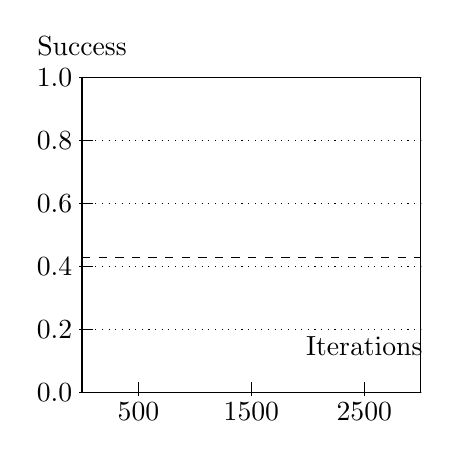
\begin{tikzpicture}[x=0.00143cm,y=4cm]
    % Draw the axes and grid lines
    \draw[-] (0,0) -- (0,1) -- (3000,1) -- (3000,0) -- cycle; 
    \draw[-,thin, dotted, ystep=0.2, xstep=3000] (0,0) grid (3000,1);
    \foreach \x in {500, 1500, 2500}  \draw [-,xshift=0](\x,4pt) -- (\x,-1pt);
    \foreach \y in {0.0,0.2,0.4,0.6,0.8,1.0}  \draw [-,yshift=0](4pt,\y) -- (-1pt,\y);
    \foreach \x/\xtext in {500/500, 1500/1500, 2500/2500} \node at (\x,0) [below] {$\xtext$};
    \foreach \y/\ytext in {0.0,0.2,0.4,0.6,0.8,1.0}  \node at (0,\y) [left] {$\ytext$};
    \node at (0,1.1) {Success};
    \node at (2500,0.15) {Iterations};
    \draw[-] plot[mark=triangle,gray,mark size=3,mark options={color=gray}] 
			file {data/test05v3gm.CP.tikzdata};
    \draw[-] plot[mark=o,gray,mark size=2,mark options={color=gray}] 
			file {data/test05v3gm.SP.tikzdata};
    % Also draw the expected convergence: 0.9^8 actions=0.43046
    \draw[dashed,-,yshift=0](0,0.43046) -- (3000,0.43046);

\end{tikzpicture}

}
\qquad
\subfigure[Structure $\T_3$]{\label{fig:T3_result}
%!TEX root = ../dsingh-aamas10-poster.tex
\begin{tikzpicture}[x=0.0032cm,y=9cm]
    % Draw the axes and grid lines
    \draw[-] (0,0) -- (0,1) -- (5000,1) -- (5000,0) -- cycle; 
    \draw[-,thin, dotted, ystep=0.2, xstep=5000] (0,0) grid (5000,1);
    \foreach \x in {1000, 2500, 4000}  \draw [-,xshift=0](\x,4pt) -- (\x,-1pt);
    \foreach \y in {0.0,0.2,0.4,0.6,0.8,1.0}  \draw [-,yshift=0](4pt,\y) -- (-1pt,\y);
    \foreach \x/\xtext in {1000/1000, 2500/2500, 4000/4000} \node at (\x,0) [below] {\xtext};
    \foreach \y/\ytext in {0.0,0.2,0.4,0.6,0.8,1.0}  \node at (0,\y) [left] {\ytext};
    \node at (0,1.15) {Success};
    \node at (4150,0.1) {Iterations};
    \draw[-,red] plot[mark=x,mark size=10,mark options={color=red}] 
			file {figs/data/testImpactvars2.CP.tikzdata};
    \draw[-,blue] plot[mark=o,mark size=6,mark options={color=blue}] 
			file {figs/data/testImpactvars2.SP.tikzdata};
    % Also draw the expected convergence: 0.9^4 actions=0.6561
    \draw[dashed,-,yshift=0](0,0.6561) -- (5000,0.6561);
	\node at (5700,0.5) {$\mathcal{T}3$};

\end{tikzpicture}

}
\caption{Agent performance under \BUL\ (circles) and \CL\ (triangles) schemes.
Each point represents results from $5$ experiment runs using a moving average of $100$ samples.}
\end{center}
\end{figure*}


In order to explore the difference between \BUL\ and \CL, we set up testbed
programs composed of several goals and plans combined in a hierarchical manner
and yielding goal-plan tree structures of different shapes. In particular, we
crafted goal-plan tree structures representing different meaningful cases of BDI
programs with one main top-level goal, i.e., the event to be resolved. In
addition, each structure enjoys the, generally desirable, \emph{coverage}
property, under which for every possible situation, (i.e., world state), there is
always a way of addressing the main goal, i.e., there is at least one successful
execution of the top-level event, provided the right plan choices are made.
Observe that such successful (plan) choices may be different for different world
states.
% , as know-how information is generally predicated on the situation it is
% applied in. %
When it comes to describing the possible (observable) world states, we have used
a set of logical (binary) propositions, representing the so-called fluent or
features of the environment that are observable to the agent (e.g., fluent
proposition $\mathit{DoorLocked}$ states whether the door is believed open or
not).
% %
Finally, we assume the agent is acting in a non-deterministic environment, in
which actions that are expected to succeed, may still fail with some (small)
probability. In most of our experiments, we assumed a $.1$ probability of
uncontrolled failure for such actions. \footnote{See Discussion section on how
our results generalize to a framework with world state built from non-binary
fluents and with more complex accounts for stochastic actions.}




The experiments consisted of posting the top-level goal repetitively
under a random world state, running the corresponding \JACK\ learning
agent, and recording whether the execution terminated successfully or
not. We calculated the average rate of success of the goal every  $20$
iterations, and investigate how this rate evolves as the agent refines
the context condition of plans. 
%
We ran the tests using both a \BUL-based agent and a \CL-based
agent, ensuring the same sampling of random world states for each
agent. 
%
% *** Could remove following sentence as we have already said this.
With \BUL, we used $k=3$ and $\epsilon=0.3$, meaning that
the context condition of a plan is considered stable at a certain
world, if we have recorded at least $3$ past experiences and the rate
of success has changed less than $0.3$ in the last executions.
%

From our set of experiments, we have selected three
hierarchical structures, that best illustrate the results that we
obtained, and the reason behind these results.
\begin{description}
\item[(Tree $\T_1$)] A structure in which \CL\ is expected to have
important advantages aver \BUL, since the former is capable of quickly
assuming a top-level plan as not good, whereas \BUL\ is expected to
devote substantial more time to get to the same conclusion. 

\item[(Tree $\T_2$)] A structure in which \BUL\ is expected to have
important advantages over \CL, since the latter may wrongly consider a
top-level plan as a failing plan whereas there is a solution encoded
under it. 

\item[(Tree $\T_3$)] A structure that is arguably a general case for
BDI systems and that provides different advantages for both \BUL\ and
\CL\ in different parts of the tree. 
\end{description}

In summary, we found that whereas the agent performance under the
\BUL\ and \CL\ approaches is comparable on the first and third cases,
the \BUL\ scheme provides substantial benefits in the second
case. What is more important, if we consider agents that may choose
not to consider a plan at all when its chances of success are believed
very low, then the \CL\ approach collapses completely whereas the
\BUL\ is robust enough to maintain performance.

% For lack of space,
% we shall only give the form of tree $\T_1$ and informally explain the characteristics of the other
% two.


In Figure \ref{fig:T1}, we show the goal-plan tree structure
$\T_1$. Initially, the agent has $20$ options to resolve the top-level
goal $G$. However, $19$ of them lead to failure (plans
$P_i'$). The benefit of using \CL\ comes from the fact that the agent
will decrease the probability of selecting each of those $19$ plans as
soon as they fail for the first time. \BUL\  however
requires several failed experiences of each of those ``bad'' top-level
options before decreasing their probability of selection---to update
the decision tree of plan $P_i'$, \BUL\ would require each of their
three subgoals to be ``stable.''
%
As we expected the \CL\ scheme does perform
better in that it achieves optimal performance faster (Figure
\ref{fig:T1_result}, cross marked). The \CL\
approach yields optimal agent performance after around $300$
iterations, whereas \BUL\ achieves such performance after around $400$
iterations\footnote{Optimal performance amounts to a $90\%$
success rate, as the environment fails with $.1$ probability and a
successful run amounts to the execution of one action ($a_1$) only. If
the environment is made fully deterministic, then agent performance
eventually achieves complete success under both schemes.}.


The second structure $\T_2$ that we considered amounts to simplifying
each plan $P_i'$ to be just a single action that always fails and
making the goal-tree hierarchy below plan $P$ more complex, that is,
deeper and with more goals.\footnote{For lack of space, we do not show
this structure.}
% \footnote{For lack of space, we do not show
% this structure, but will be included in the final version.}
%
Under such hierarchy, the agent needs to make four correct plan
choices to result in a successful execution; there are also many
chances for the agent to fail under $P$.
%
Although one would expect \BUL\ to yield better agent performance than
\CL, the difference is enormous. Figure \ref{fig:T2_result} shows
that while the \BUL\ approach, achieves optimal performance in around
$100$ iterations, the \CL\ scheme, requires around $5000$ execution
experiences.  
%
The reason is clear: since there are more chances to fail plan $P$
initially, \CL\ marks this plan ``bad,'' causing plans $P_i'$ (which
are all non-working) to be selected at least once in preference to
trying $P$ again. On the other hand, \BUL\ would not consider $P$
``bad'' even when failing it, since it is aware that decisions made 
below were not informed enough. Consequently $P$ will continue to be
explored with equal likelihood to the $P_i'$.
% *** Sentence below could be cut - its an aside...
%
As a matter of fact,
provided adequate parameters are used for checking stability, \BUL\
would only record failed execution traces in plan $P$ if the
environment happened to fail unexpectedly: if the decisions were
informed and the environment cooperated, then the execution is
expected to succeed. 
%
Notice that optimal behavior amounts to less than a $75\%$ rate of
success, since the agent needs to ultimately perform four actions,
each of them having a probability of success of $90\%$ when performed
in the real world. 

Let us now consider the third hierarchical structure $\T_3$, depicted
in Figure \ref{fig:T3}. In this case, the top-level goal $G$ has
five relevant plans, which are all ``complex,'' that is, they all have
several levels and multiple goals and plans. However, only one
particular path in this hierarchy will lead to a successful 
execution for a particular world state. 
Among other things, this means that at the top-level the agent ought
to select the right plan, all the other four plans are bound to fail
eventually. 
%
We argue that this is the typical case in most BDI agent systems, in
that for each goal, the agent may have several strategies, but each
one is crafted to cover uniquely a particular subset of states.
%
From the two learning approaches we are considering, structure $\T_3$
provides advantages for both of them, in different parts of the
tree. The \CL\ scheme is expected to learn faster the inadequacy 
of the four non-working top-level programs, but the \BUL\ would better
explore, and find a solution, within the working top-level plan.
%
This balance is corroborated by the fact that both agents have
comparable performance, with \BUL\ yielding improved behavior slightly
quicker (see Figure \ref{fig:T1_result}, circle marked). 

However, we are currently considering all plans as potentially
applicable and worth trying - even when there is a very low chance of
success. Given that executing a plan is often not cost-free in real
systems, it is likely that the plan selection mechanism would in fact
not execute plans with too low a probability of success. This would
presumably hurt \CL.
% 
In order to demonstrate this we modified the probabilistic plan
selection explained in Section \ref{sec:framework} so that the \JACK\
agent does not consider plans whose chance of success are below 0.2.
In this experiment we also removed the non-determinism---actions
always fail or succeed in each world state.\footnote{Managing the
non-determinism without continuing to, with some probability, try all
plans, requires a more sophisticated mechanism than a simple
probability check, to avoid randomly cutting off options that happen
to have failed on one iteration. However in the interests of
simplicity we deal with the simplified case.}
%
The differences, shown in Figure \ref{fig:T2_result} are striking.

Using the structure 
$\T_3$ we  found that whereas \BUL\ maintains its performance (and in
fact slightly improves, as failing leaf plans are discarded earlier
than before thus reaching optimal performance around $100$
iterations), the \CL\ approach is never able to learn and eventually
is guaranteed to always fail the top-level goal.

The explanation for this wrong behavior under \CL\ is as
follows. Initially, the agent tries all top-level plans for the
top-level goal. Because of their complexity, it is extremely unlikely
that the set of correct choices are made randomly. Thus their
executions fail.
This causes \CL\ to decrease the feasibility of all plans
tried, including the top-level ones. As this will likely happen
for several iterations, eventually all plans for a goal reach a probability of
success lower than required, thus
running out of options, failing the goal in question, and propagating
the failure up in the hierarchy. Eventually, the top-level plans end
up with low expectations of success and are ruled out.
This will give no options to try and the goal will always
fail.\footnote{Such behavior does not arise in the original
system because even if all plans have extremely low success chances,
the agent would pick one anyway. As a result, the successful path
would be eventually be found and plans' context conditions would start
``recovering.''}

We conclude then that overall \BUL\ clearly exhibits more robust
behaviour. In addition, in some structures \CL\ can pay significant
costs, by considering some strategies as not viable too early. In
those structures where \BUL\ performs worse, the difference is
relatively small. 

\begin{figure}
\begin{center}
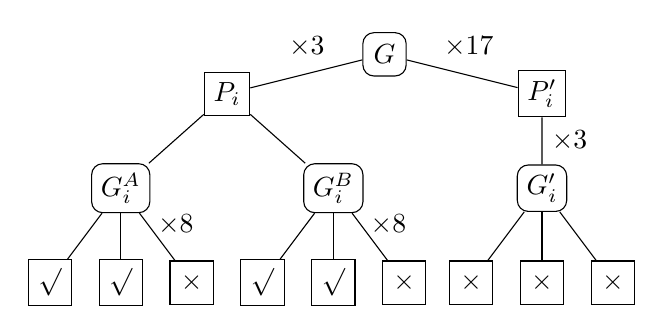
\begin{tikzpicture}[level distance=1.2cm]

\tikzstyle{planbox}=[draw,minimum height=0.55cm,minimum width=0.55cm]
\tikzstyle{goalbox}=[draw,rounded corners,minimum height=0.55cm,minimum width=0.55cm]

\tikzstyle{level 1}=[sibling distance=4cm,level distance=0.5cm] 
\tikzstyle{level 2}=[sibling distance=2.7cm,level distance=1.2cm]
\tikzstyle{level 3}=[sibling distance=.9cm]
\tikzstyle{level 4}=[sibling distance=1cm]

\node[goalbox] (T) {$G$}
   child[solid] {node[planbox] (1) {$P_i$}
      	child {node[goalbox] (11) {$G_i^A$}
			child {node[planbox] {$\surd$}
			}
			child {node[planbox] {$\surd$}
			}
			child {node[planbox] {$\times$}
				edge from parent node[right,near start] {$\times 8$}
			}
	  	}
      	child {node[goalbox] (11) {$G_i^B$}
			child {node[planbox] {$\surd$}
			}
			child {node[planbox] {$\surd$}
			}
			child {node[planbox] {$\times$}
				edge from parent node[right,near start] {$\times 8$}
			}
	  	}
	edge from parent node[above left, near start] {$\times 3$}
   }
   child[solid] {node[planbox] (2) {$P_i'$}
      child {node[goalbox] (22) {$G_i'$} 
	child {node[planbox] {$\times$}}
	child {node[planbox] {$\times$}}
	child {node[planbox] {$\times$}}
	edge from parent node[right] {$\times 3$}
	}
   edge from parent node[above right,near start] {$\times 17$}};

% \draw (T) -- (1) node (aux1) [coordinate,midway]{};
% \draw (T) -- (2) node (aux2) [coordinate,midway]{};
% \draw (aux1) .. controls +(0.3,-0.3) and +(-0.3,-0.3).. (aux2)
% 			node[midway,above] {OR};

% \draw (1) -- (11) node (aux21) [coordinate,midway]{};
% \draw (1) -- (12) node (aux23) [coordinate,midway]{};
% \draw (aux21) .. controls +(0.25,-0.25) and +(-0.25,-0.25).. (aux23)
% 			node[midway,above] {AND};

% \node[below left of=T,text width=2cm,xshift=-3cm] (label)
% 		{$P_i$: plan \\ $G_i$: goals \\ $SG_i$: sub-goals};
\end{tikzpicture}

\end{center}
\caption{Goal-plan tree hierarchical structure $\T_1$. To succeed, an agent is thus required to make
two correct choices, including selecting $P$ at the top-level.}
% \caption{Goal-plan tree hierarchical structure $\T_1$. Leaf plans are assumed to succeed or fail
% when executed in the environment. An edge with a label $\times n$ states that there are $n$ edges
% of such type. As a result, goals $G$ and $G_P$ have $20$ relevant plans each. To succeed, an agent
% is thus required to make two correct choices, including selecting $P$ at the top-level.}
\label{fig:T1}
\end{figure}


\begin{figure}
\begin{center}
%!TEX root = ../dsingh-aamas10.tex
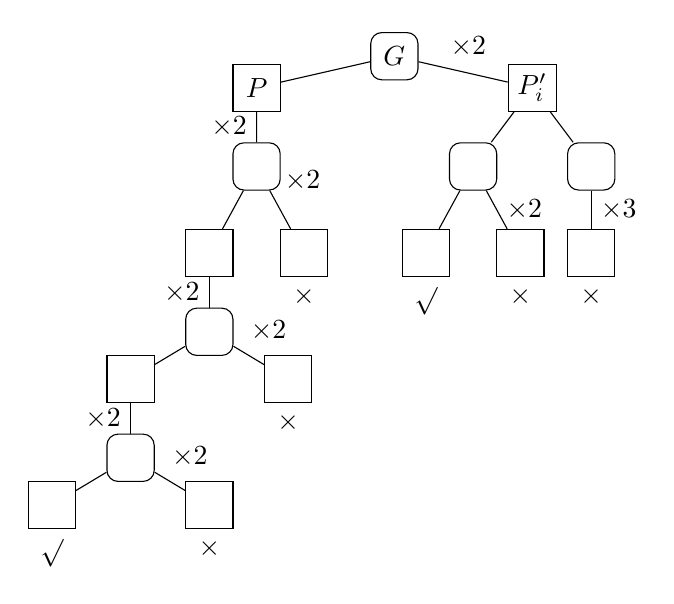
\begin{tikzpicture}[level distance=1.2cm]
\tikzstyle{txt}=[scale=.9]

\tikzstyle{succ}=[label=below:$\surd$]
\tikzstyle{fail}=[label=below:$\times$]


\tikzstyle{planbox}=[draw,minimum height=0.6cm,minimum width=0.6cm]
\tikzstyle{goalbox}=[draw,rounded corners,minimum height=0.6cm,minimum width=0.6cm]

\tikzstyle{level 1}=[sibling distance=3.5cm,level distance=0.4cm] 
\tikzstyle{level 2}=[sibling distance=1.5cm,level distance=1.0cm]
\tikzstyle{level 3}=[sibling distance=1.2cm,level distance=1.1cm]
\tikzstyle{level 4}=[sibling distance=1.2cm,level distance=1.0cm]
\tikzstyle{level 5}=[sibling distance=2.0cm,level distance=0.6cm]
\tikzstyle{level 6}=[sibling distance=1.2cm,level distance=1.0cm]
\tikzstyle{level 7}=[sibling distance=2.0cm,level distance=0.6cm]
\tikzstyle{level 8}=[sibling distance=1.2cm,level distance=1.0cm]

\node[goalbox] (T) {$G$}
   child[solid] {node[planbox] (1) {$P$}
      child {node[goalbox] (11) {\phantom{$G$}}
		child {node[planbox] {\phantom{$P$}}
			child {node[goalbox] {\phantom{$G$}}
				child {node[planbox] {\phantom{$P$}}
					child {node[goalbox] {\phantom{$G$}}
						child {node[planbox,succ] {\phantom{$P$}}}
						child {node[planbox,fail] {\phantom{$P$}}
							edge from parent node[above right,near start] {$\times 2$}
						}
						edge from parent node[left] {$\times 2$}
					}
				}
				child {node[planbox,fail] {$\phantom{P}$}
					edge from parent node[above right,near start] {$\times 2$}
				}
		               edge from parent node[left] {$\times 2$}
			}
		}
		child {node[planbox,fail] {\phantom{$P$}}
			edge from parent node[above right,near start] {$\times 2$}
		}
               edge from parent node[left] {$\times 2$}
	}
   }
   child[solid] {node[planbox] (2) {$P_i'$}
      	child {node[goalbox] (11) {\phantom{$G$}}
			child {node[planbox,succ] {$\phantom{P}$}}
			child {node[planbox,fail] {$\phantom{P}$} 
		               edge from parent node[right] {$\times 2$}
			}
	}
      	child {node[goalbox] {\phantom{$G$}}
			child {node[planbox,fail] {$\phantom{P}$} 
		               edge from parent node[right] {$\times 3$}
			}
	}
	edge from parent node[above right, near start] {$\times 2$}
};
\end{tikzpicture}



\end{center}
\caption{Goal-plan tree hierarchical structure $\T_2$.}
\label{fig:T2}
\end{figure}


